\documentclass[8pt,a4paper]{article}
\pagestyle{plain}
\usepackage{fullpage}
\usepackage{indentfirst} %首段縮排
\usepackage[top=1.5cm, bottom=1.5cm, left=0.5cm, right=0.5cm]{geometry} %伍錫志
\usepackage{amsmath,amsthm,amsfonts,amssymb,amscd,longtable}
\usepackage{lastpage}
\usepackage{enumerate}
\usepackage{fancyhdr}
\usepackage{mathrsfs}
\usepackage{mathtools}
\usepackage{longtable}
\usepackage{bookmark}
\usepackage{multicol}
\usepackage[dvipsnames]{xcolor} % high light text
\usepackage{xcolor}
\usepackage{verbatim}
\usepackage{float}  % in order to use H for figure position
\usepackage{graphicx}
\DeclareGraphicsExtensions{.pdf,.jpg,.png,.mps} % Portable Document Format,
%\usepackage{luacode}  % This can not let Reference to be showed by Butters
\usepackage{multirow}
\usepackage{makecell}
\usepackage{listings}
\usepackage{multicol}
\usepackage{hyperref}
\usepackage{graphicx}
\usepackage{subfigure}
\usepackage{caption}
\usepackage{xeCJK} %For Traditional Chinese in XeLaTeX
\setCJKmainfont{MingLiU} %For Traditional Chinese in XeLaTeX
\setCJKsansfont{Microsoft JhengHei} %For Traditional Chinese in XeLaTeX

% BibTeX
%\usepackage{bibentry} %Function unknown added by Per Sahlholm
%\usepackage[round,authoryear]{natbib} %Nice author (year) citations
\usepackage[square,numbers]{natbib} %Nice numbered citations
%\usepackage{cite} % Make references as [1-4], not [1,2,3,4]
%\newcommand{\bibspace}{\vspace{2mm}}
\bibliographystyle{unsrtnat} % Unsorted bibliography by Butters
%\bibliographystyle{plainnat} %Choose for including URLs   %Commented by Butters
%\bibliographystyle{unsrt} 
%\bibpunct{[}{]}{,}{y}{,}{,}
%\renewcommand{\bibsection}{} %Removes the References chapter title
%\usepackage[numbib,notlof,notlot,nottoc]{tocbibind} %Adds number to bibliography

\let\ds\displaystyle
\usepackage[shortlabels]{enumitem}
%\pagenumbering{gobble} % Remove page number
\pagestyle{plain}
\hypersetup{
  colorlinks=true,
  linkcolor=blue, 
  citecolor=blue,% new
  linkbordercolor={0 0 1}
}


\begin{document}
%makecell setting for fonts, spacing etc.

\title{\bf{ Data mining Project 2 }}
\date{}
\author{N16074988 伍錫志}

\maketitle

\section*{Outline} 
\label{sec:Outline}
\bookmark[level=chapter,page=\arabic{page}]{Outline}

\begin{enumerate}
    \item Design rule and genrate data
    \item Decision tree parameter settings
    \item Result analysis
    \item Decision stucture analysis (gini criterion)
    \item Decision stucture analysis (entropy criterion)
    \item Discussion
\end{enumerate}

\section*{Design rule and genrate data} 
\label{sec:Design rule and genrate data}
\bookmark[level=chapter,page=\arabic{page}]{Design rule and genrate data}
Textbook:\cite{han2011data}
總共有21個 attributes/features,設計圖如 Figure \ref{fig:generation_rule}:
\begin{figure}[H]
    \begin{center}
        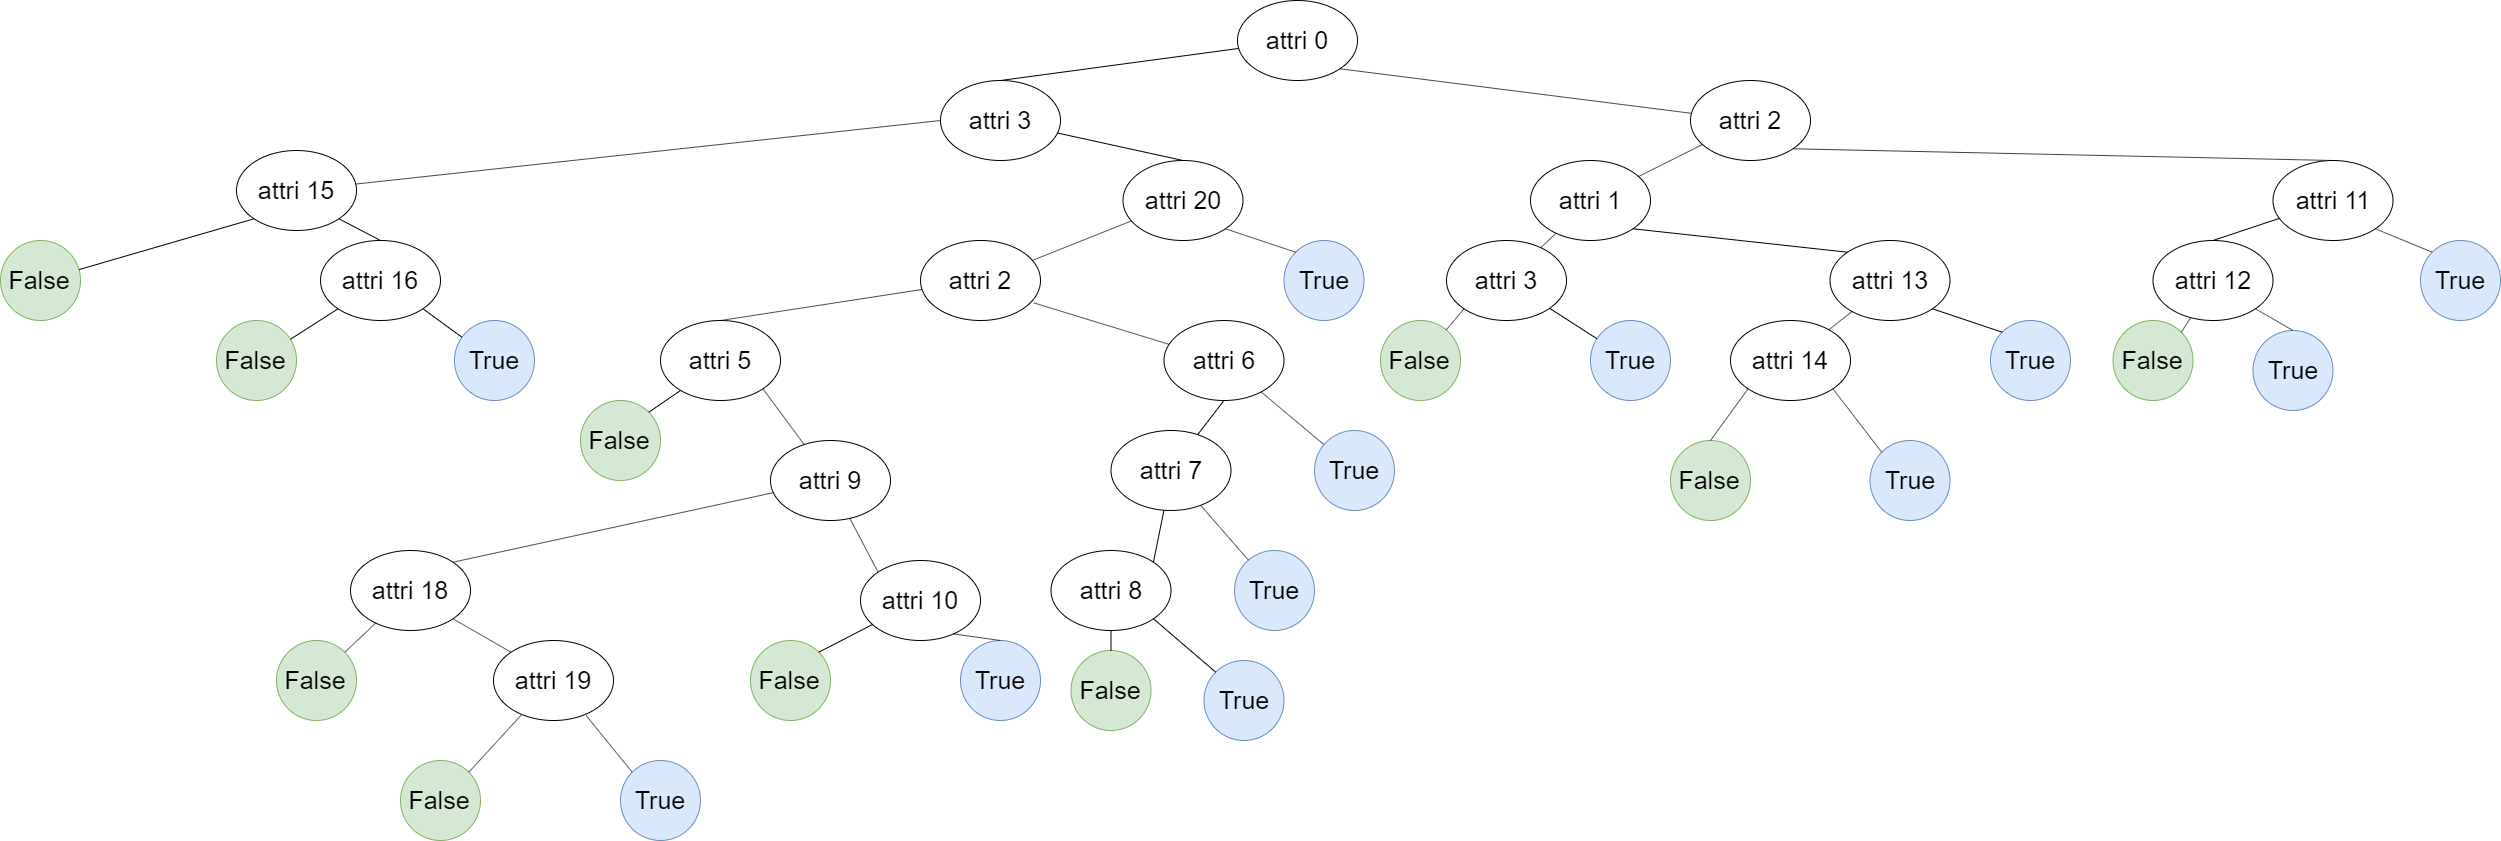
\includegraphics[width=500pt]{generation_rule.png}
        \caption{My Generation Rule}
        \label{fig:generation_rule}
    \end{center}
\end{figure}

在產生的數據的過程中,我利用隨機的方式來產生每個特徵的值(True or False)。此外,為了觀察數據量對於分類器的成效,決定分別產生100, 500, 1000, 2500, 5000, 10000筆資料。\\

\section*{Decision tree parameter settings} 
\label{sec:Decision tree parameter settings}
\bookmark[level=chapter,page=\arabic{page}]{Decision tree parameter settings}

決策樹的參數主要可以調樹的深度、節點評估方式(gini or entropy)。因此,實驗設置了5種深度來來做比較並將輸入的資料以7:3的比例分別做為訓練和測試,並且觀察不同結構時不同資料量對其的影響大小,將結果輸出成圖表來進行分析。最後,再利用graphviz這套軟體將決策樹的結果以視覺化的方式呈現出來。\\



\section*{Result analysis} 
\label{sec:Result analysis}
\bookmark[level=chapter,page=\arabic{page}]{Result analysis}

Accury of different tree structure wtith different input numbers:\\

\begin{table}[H]
    \centering
    \begin{tabular}{cccccccc}
        \hline
     & 100 & 500 & 1000 & 2500 & 5000 & 10000 & 20000 \\ \hline \\
    3 & 0.633333 & 0.733333 & 0.786667 & 0.750667 & 0.762667 & 0.756333 & 0.761667 \\
    4 & 0.666667 & 0.893333 & 0.896667 & 0.901333 & 0.894 & 0.871333 & 0.888333 \\
    5 & 0.833333 & 0.873333 & 0.936667 & 0.866667 & 0.928 & 0.925333 & 0.906333 \\
    6 & 0.566667 & 0.78 & 0.903333 & 0.976 & 0.961333 & 0.982333 & 0.965833 \\
    no limit & 0.766667 & 0.953333 & 0.953333 & 0.996 & 1 & 1 & 1
    \end{tabular}
    \caption{gini criterion}
    \label{tab:gini_table}
\end{table}

\begin{table}[H]
    \centering
    \begin{tabular}{cccccccc}
        \hline
        & 100 & 500 & 1000 & 2500 & 5000 & 10000 & 20000 \\ \hline \\
    3 & 0.633333 & 0.733333 & 0.786667 & 0.750667 & 0.762667 & 0.756333 & 0.761667 \\
    4 & 0.666667 & 0.893333 & 0.896667 & 0.901333 & 0.894 & 0.871333 & 0.888333 \\
    5 & 0.833333 & 0.873333 & 0.936667 & 0.866667 & 0.928 & 0.925333 & 0.906333 \\
    6 & 0.633333 & 0.753333 & 0.903333 & 0.976 & 0.961333 & 0.982333 & 0.965833 \\
    no limit & 0.766667 & 0.953333 & 0.956667 & 0.996 & 1 & 1 & 1
    \end{tabular}
    \caption{entropy criterion}
    \label{tab:entropy_table}
\end{table}

從Table \ref{tab:gini_table}, \ref{tab:entropy_table} 中我們可以發現,隨著資料量上升時,決策樹的分類的準確度要較高,而當樹的深度越深時準確率也相對較高,這也可以驗證了我所設計的樹狀結構是無法用較低層數的結構來呈現的所以在低深度的準確度上能會有所缺失。
此外,雖然這兩張圖表所用的計算準則不同,但結果卻非常接近,我認為是由於計算準則的過程只有在數值程度上的不同並不會影響其分類的依據因此在這一個例子中所產生的結果都會一致。\\



\section*{Decision stucture analysis (gini criterion)} 
\label{sec:Decision stucture analysis (gini criterion)}
\bookmark[level=chapter,page=\arabic{page}]{Decision stucture analysis (gini criterion)}

\begin{figure}[H]
    \begin{center}
        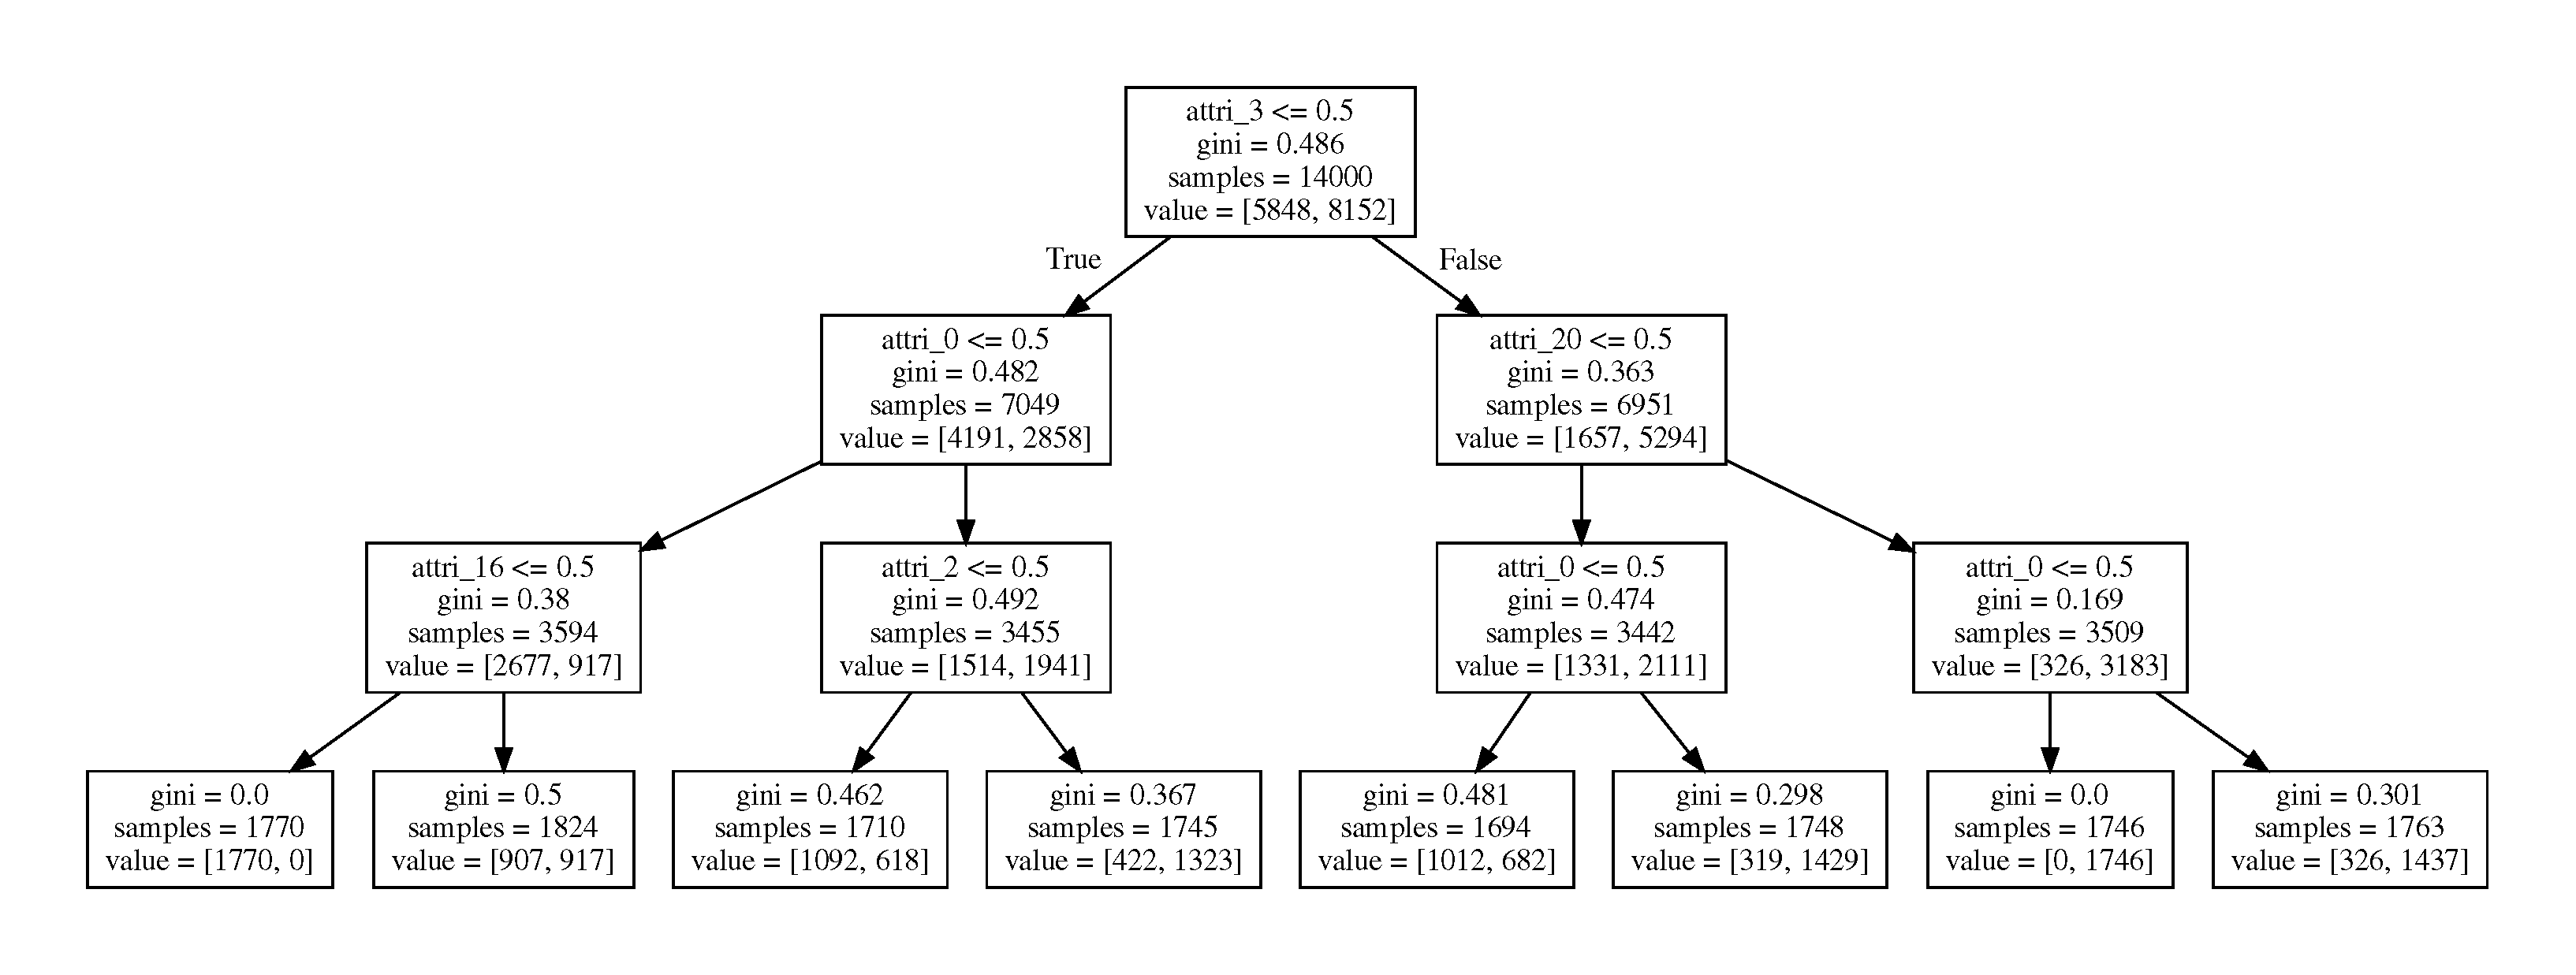
\includegraphics[width=550pt]{decision_tree_depth_m1_3.png}
        \caption{max-depth=3}
        
    \end{center}
\end{figure}

\begin{figure}[H]
    \begin{center}
        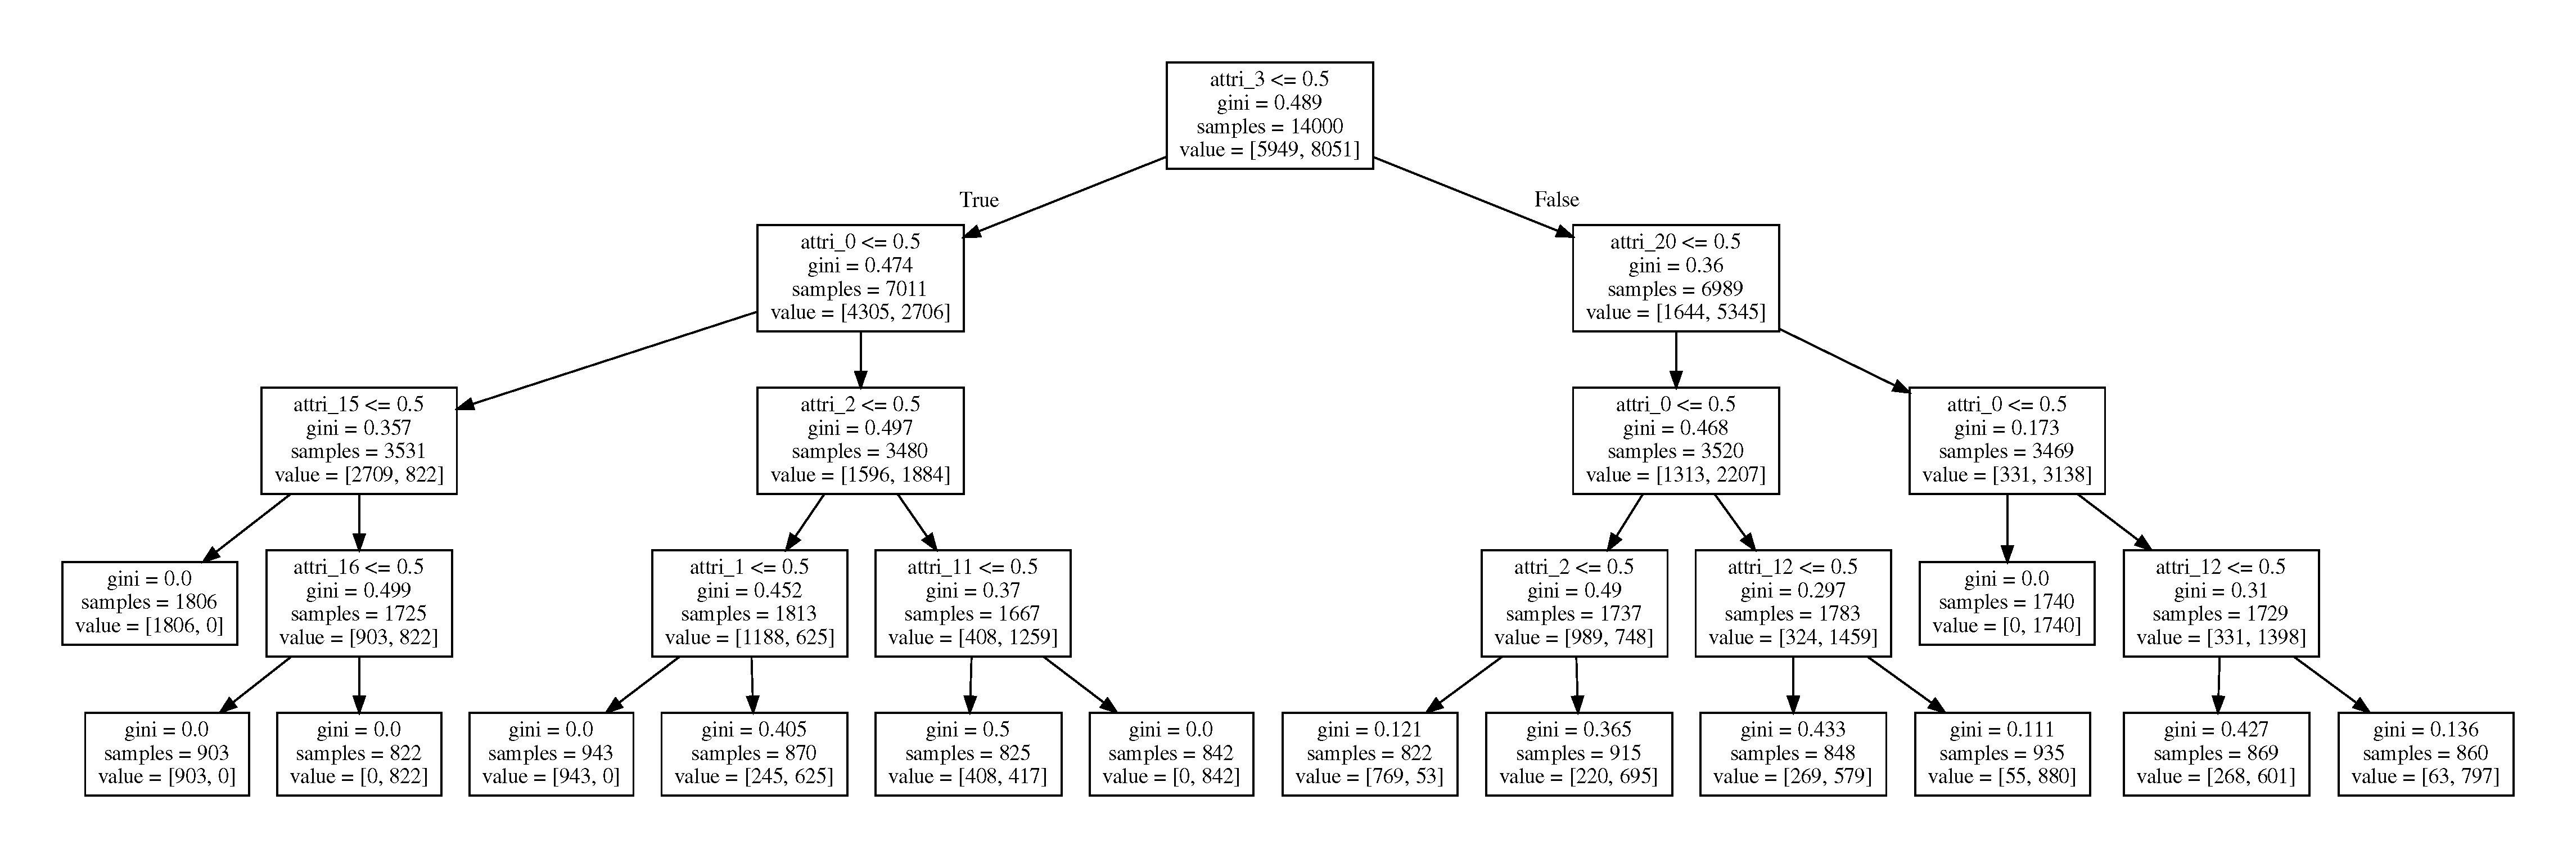
\includegraphics[width=550pt]{decision_tree_depth_m1_4.png}
        \caption{max-depth=4}
        
    \end{center}
\end{figure}

\begin{figure}[H]
    \begin{center}
        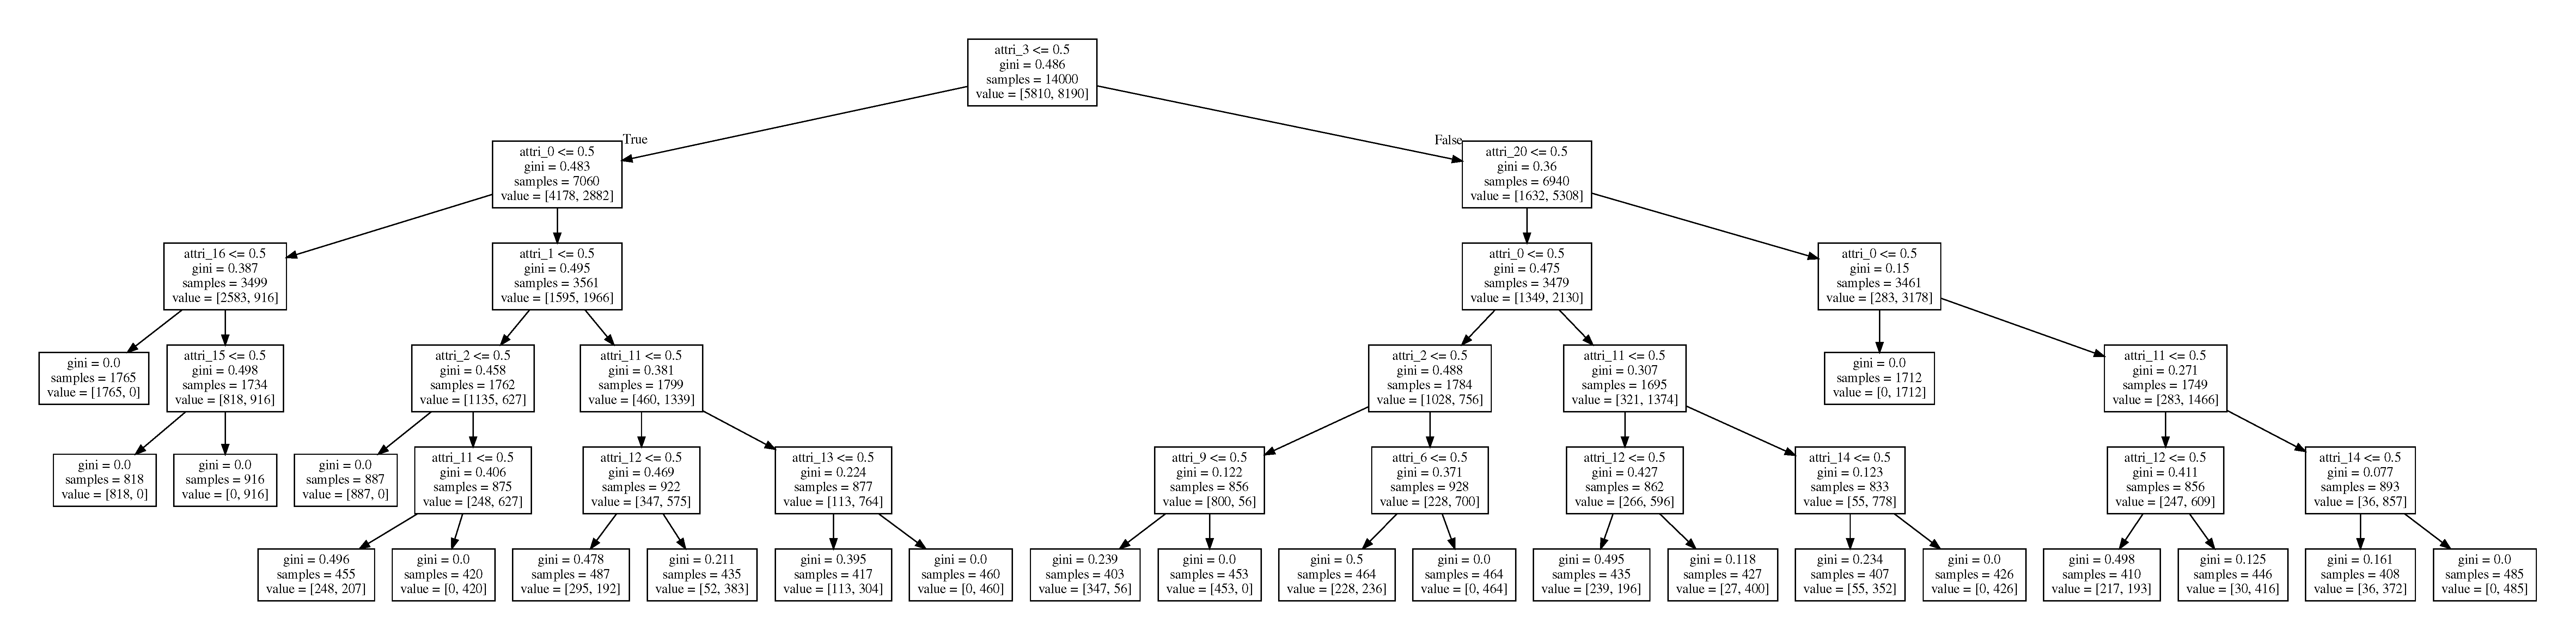
\includegraphics[width=550pt]{decision_tree_depth_m1_5.png}
        \caption{max-depth=5}
        
    \end{center}
\end{figure}

\begin{figure}[H]
    \begin{center}
        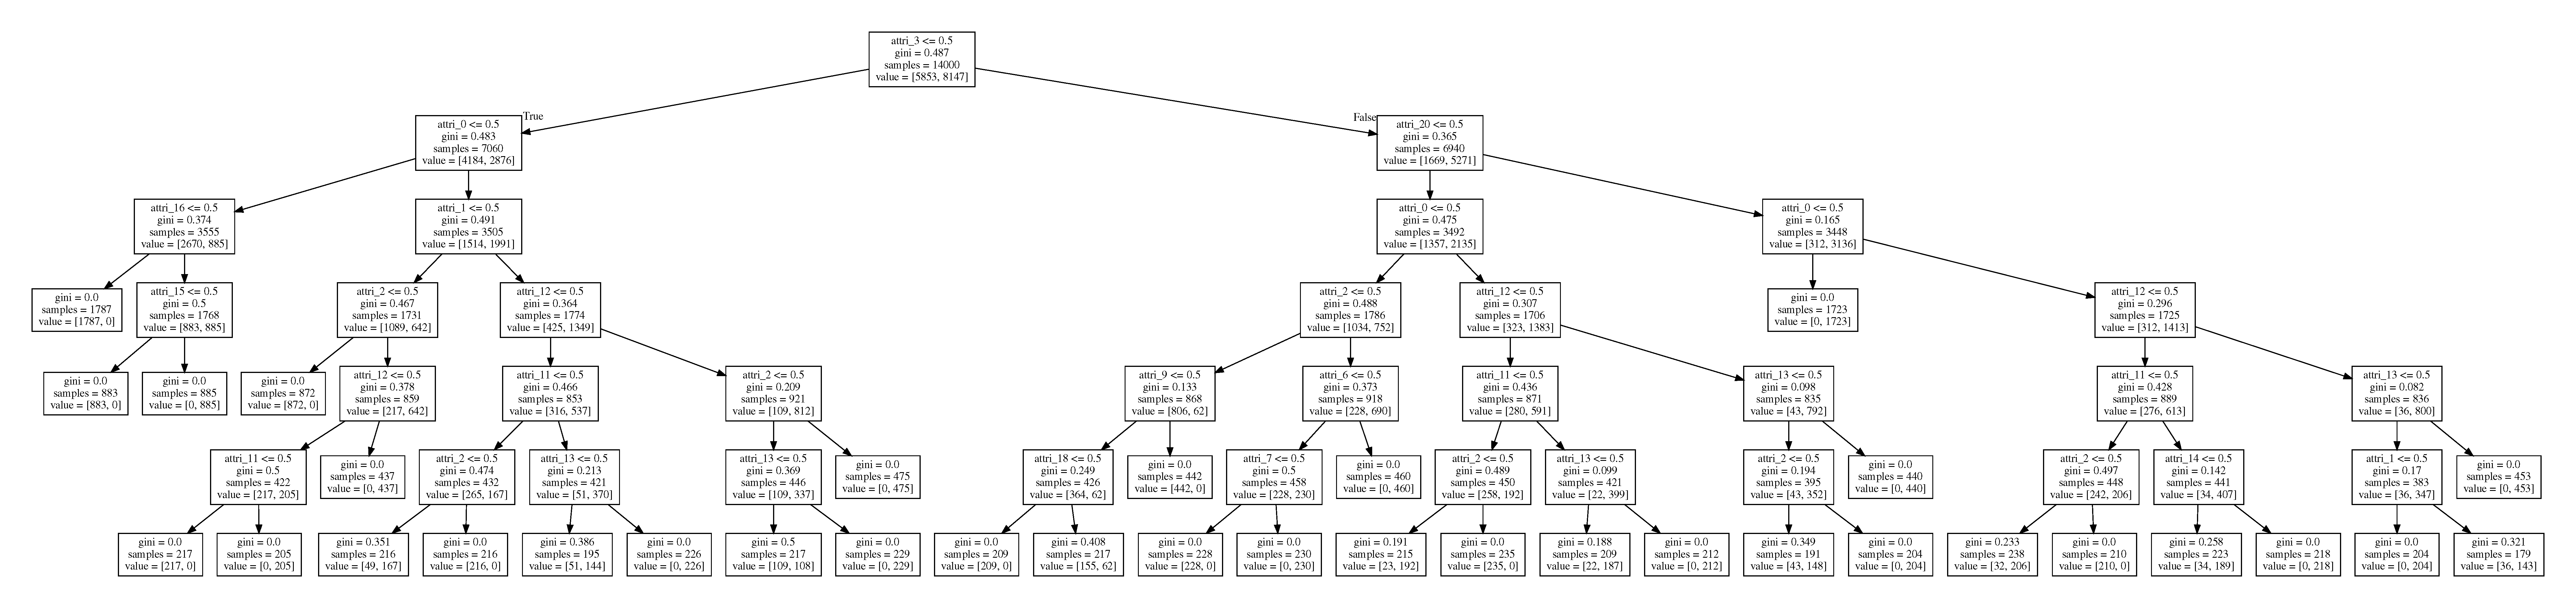
\includegraphics[width=550pt]{decision_tree_depth_m1_6.png}
        \caption{max-depth=6}
        
    \end{center}
\end{figure}

\begin{figure}[H]
    \begin{center}
        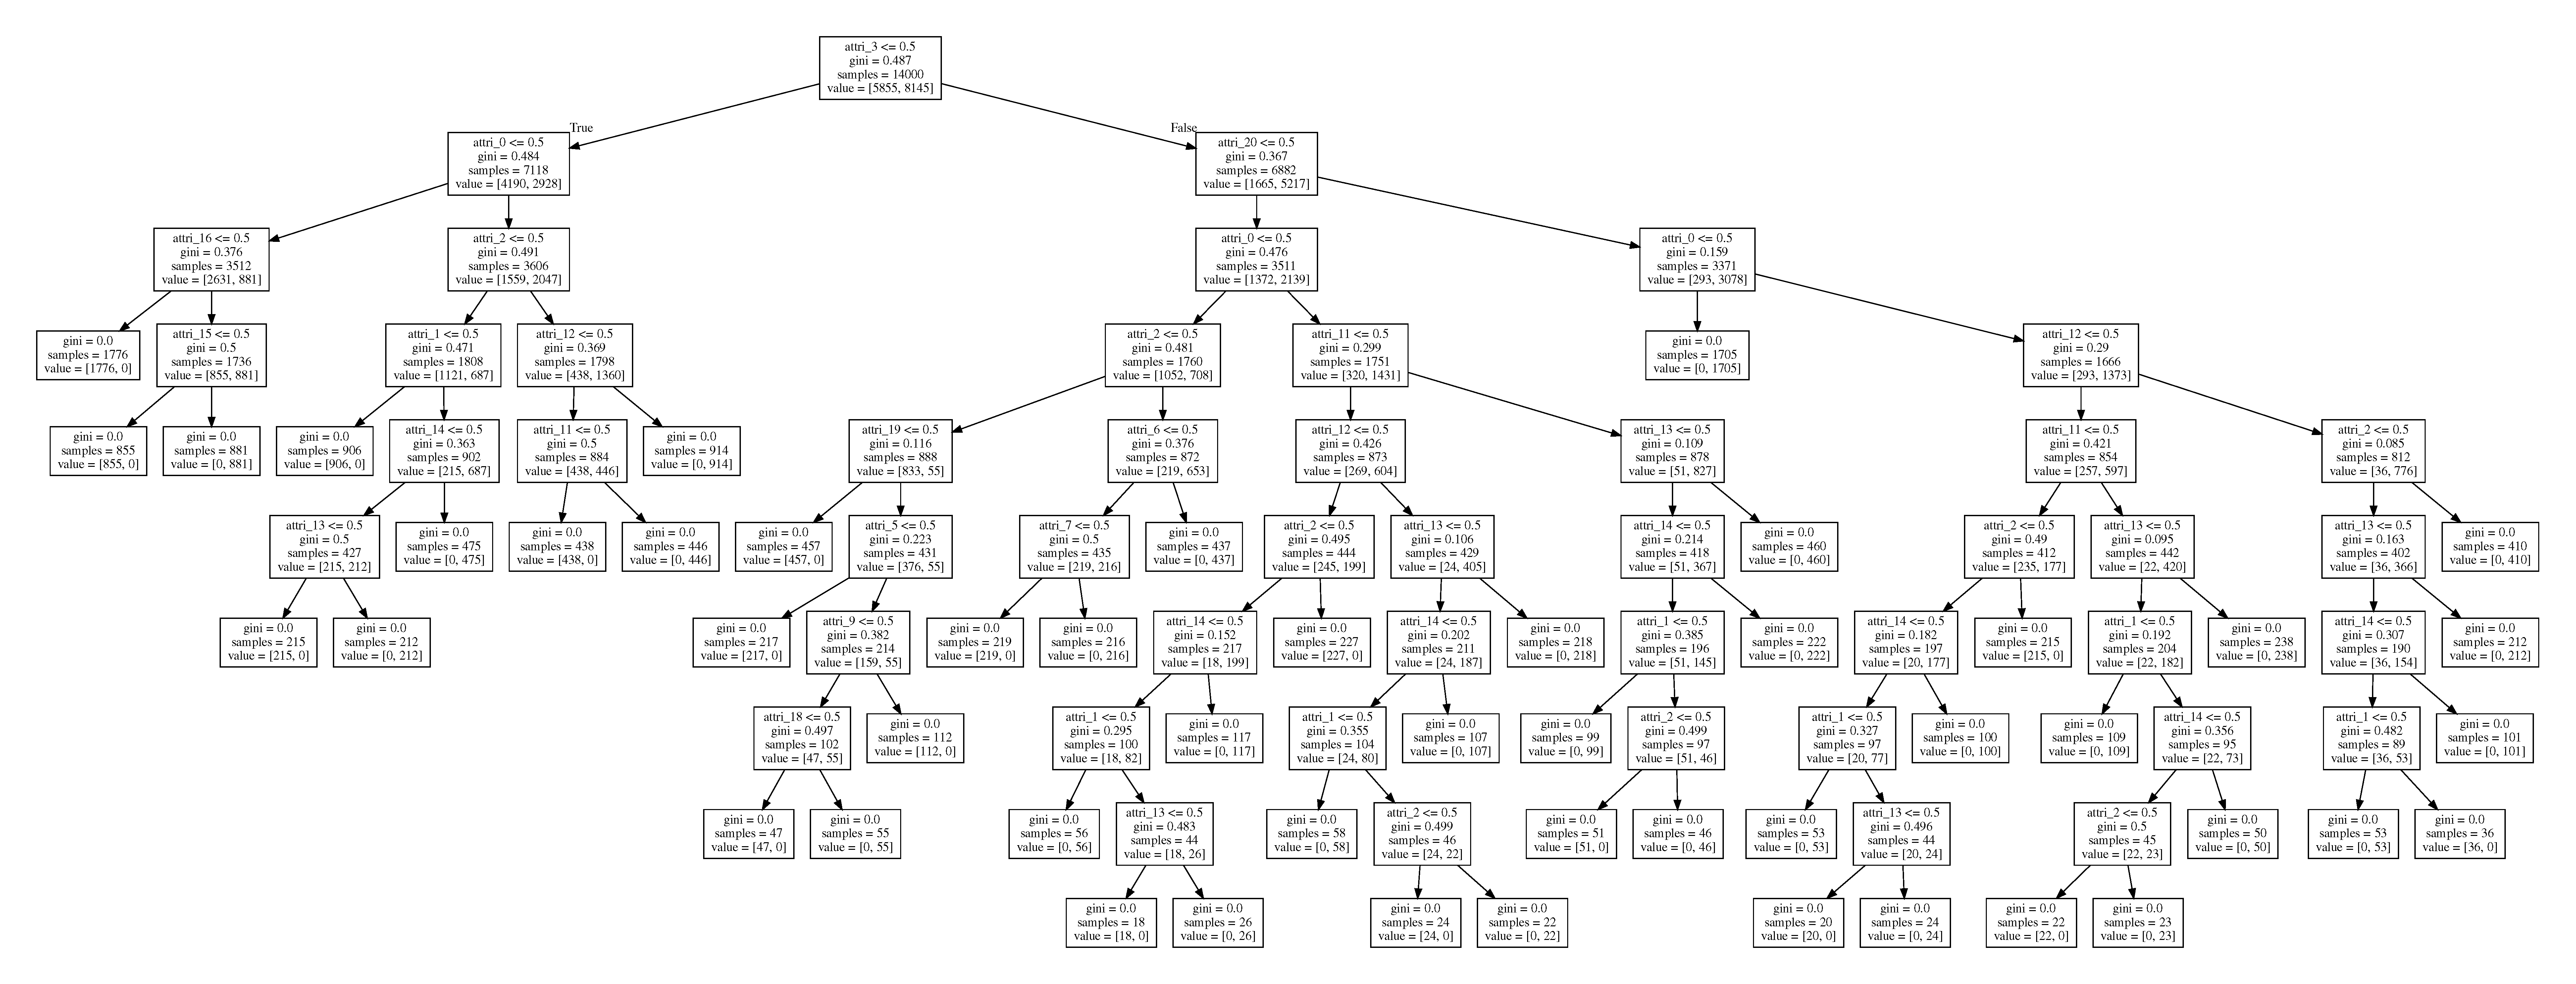
\includegraphics[width=550pt]{decision_tree_depth_m1_7.png}
        \caption{max-depth=7}
        
    \end{center}
\end{figure}


\section*{Decision stucture analysis (entropy criterion)} 
\label{sec:Decision stucture analysis (entropy criterion)}
\bookmark[level=chapter,page=\arabic{page}]{Decision stucture analysis (entropy criterion)}

\begin{figure}[H]
    \begin{center}
        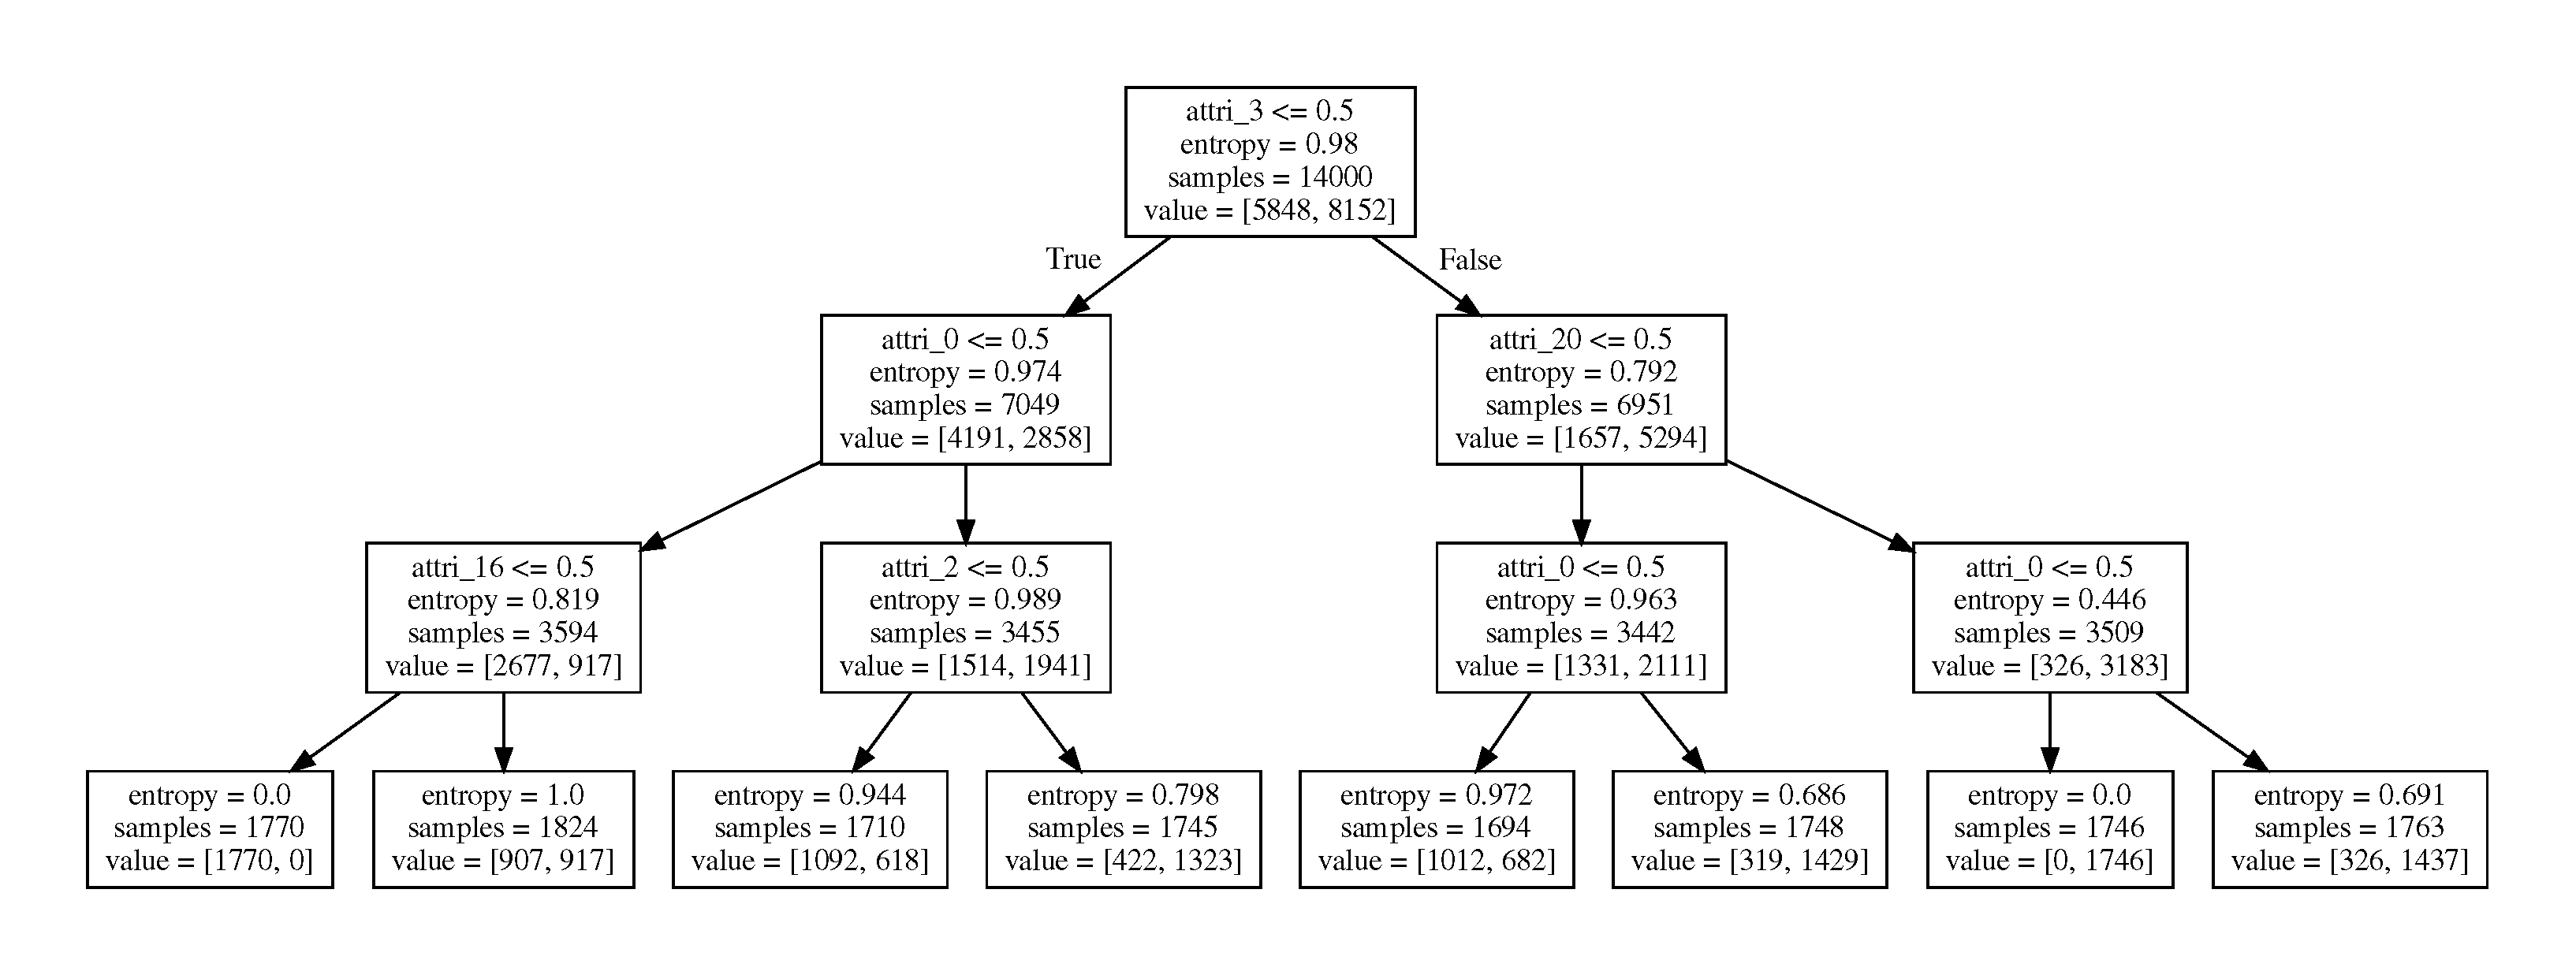
\includegraphics[width=550pt]{decision_tree_depth_m2_3.png}
        \caption{max-depth=3}
        
    \end{center}
\end{figure}


\begin{figure}[H]
    \begin{center}
        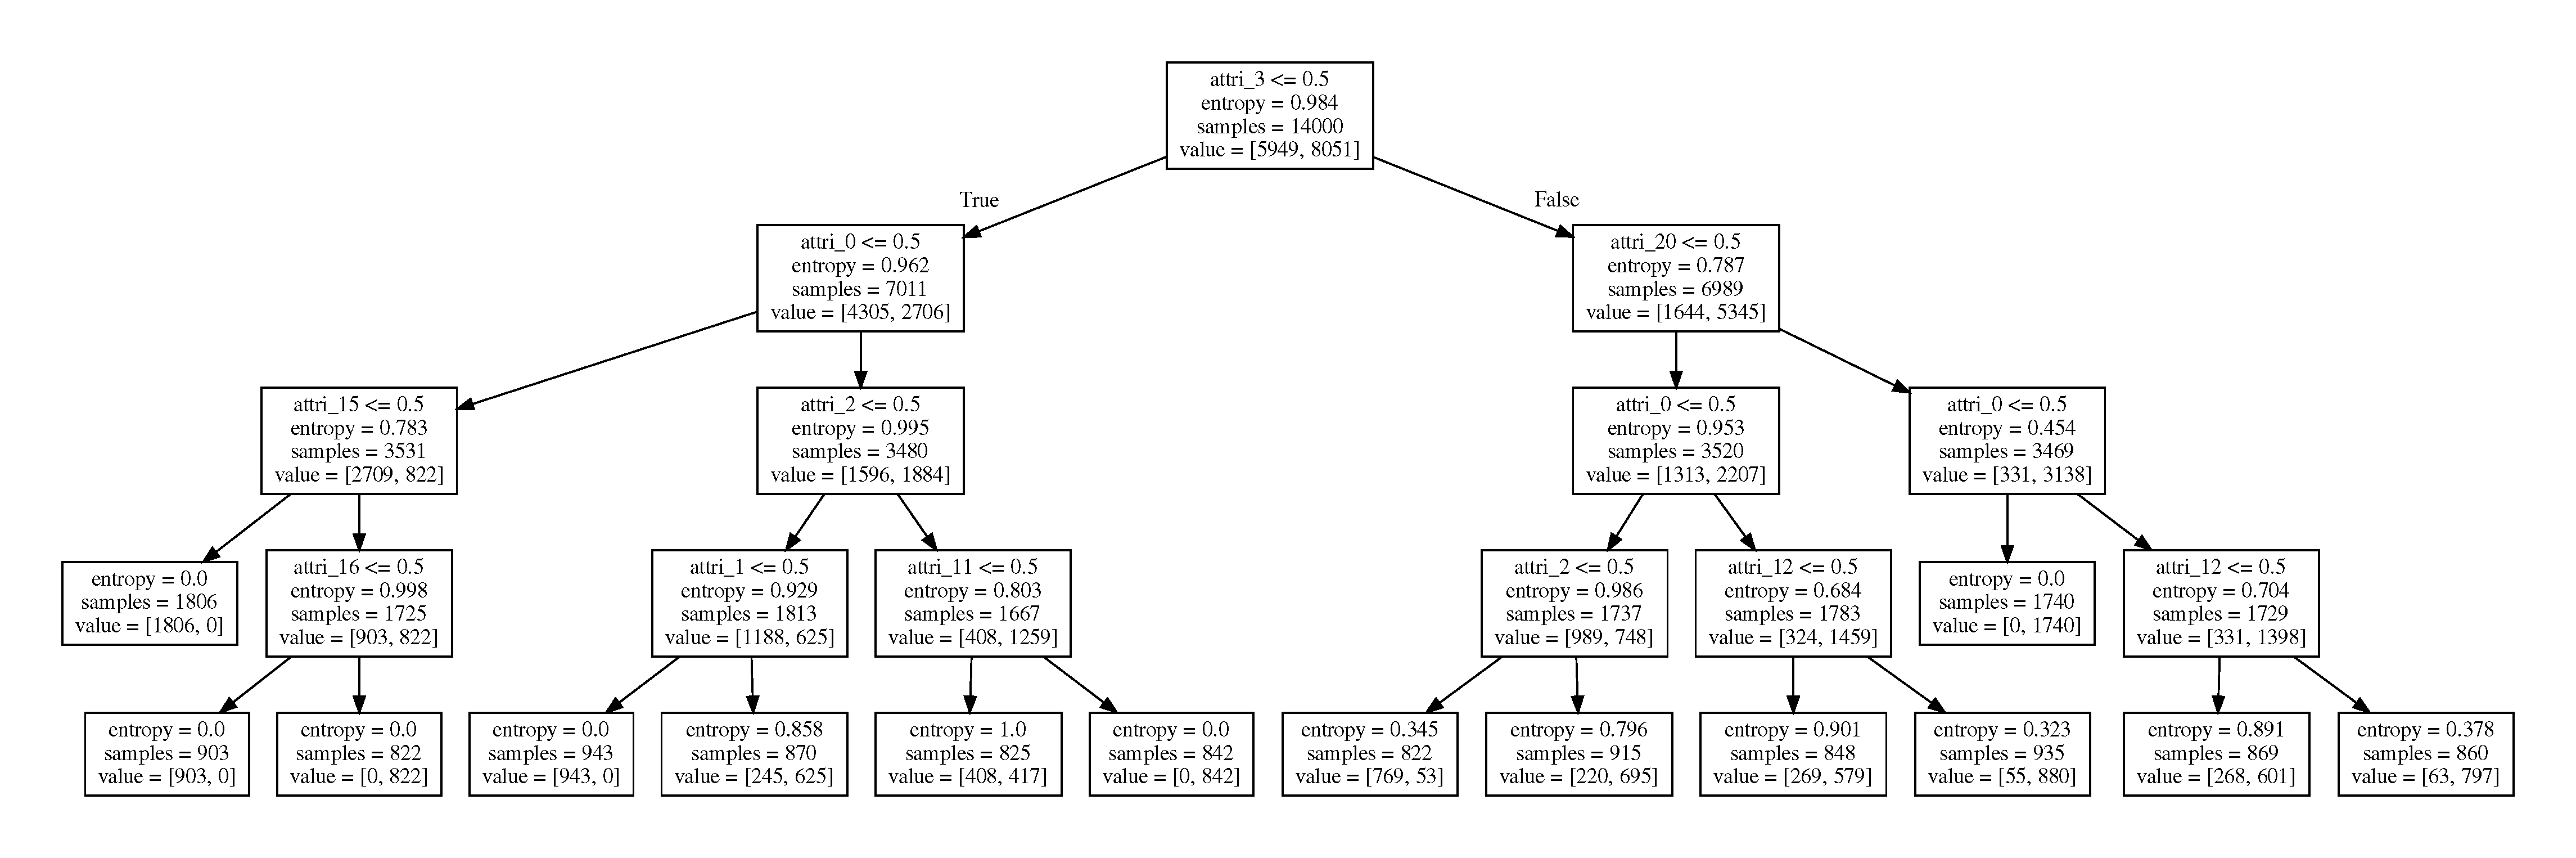
\includegraphics[width=550pt]{decision_tree_depth_m2_4.png}
        \caption{max-depth=4}
        
    \end{center}
\end{figure}


\begin{figure}[H]
    \begin{center}
        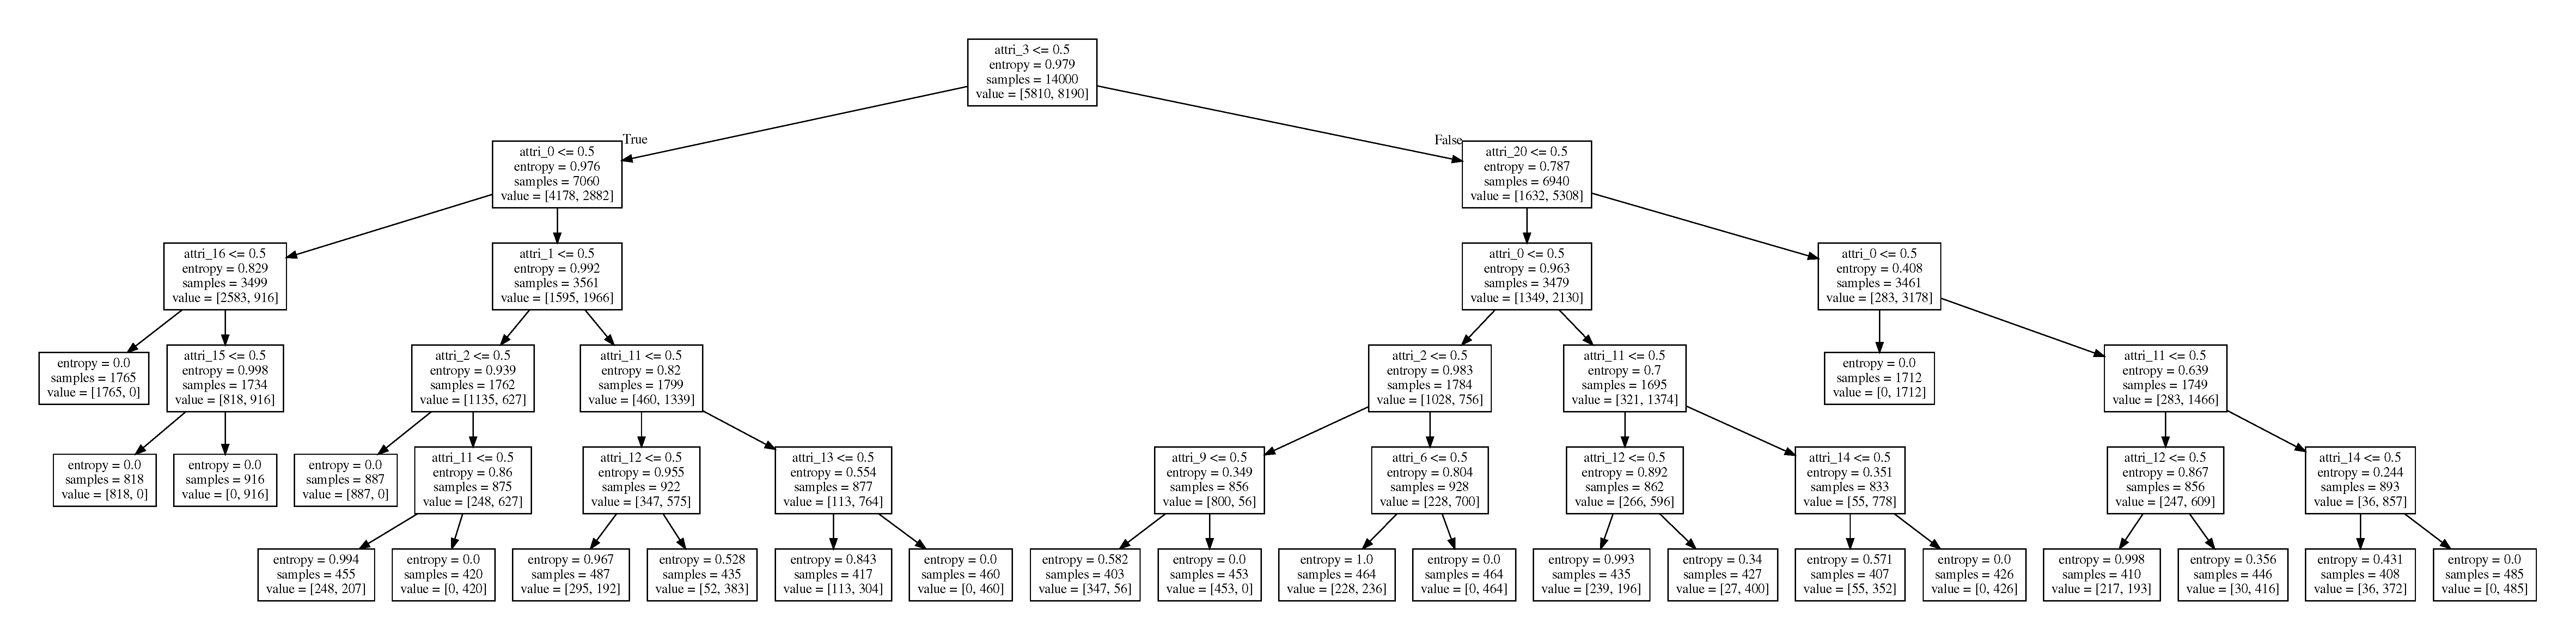
\includegraphics[width=550pt]{decision_tree_depth_m2_5.png}
        \caption{max-depth=5}
        
    \end{center}
\end{figure}


\begin{figure}[H]
    \begin{center}
        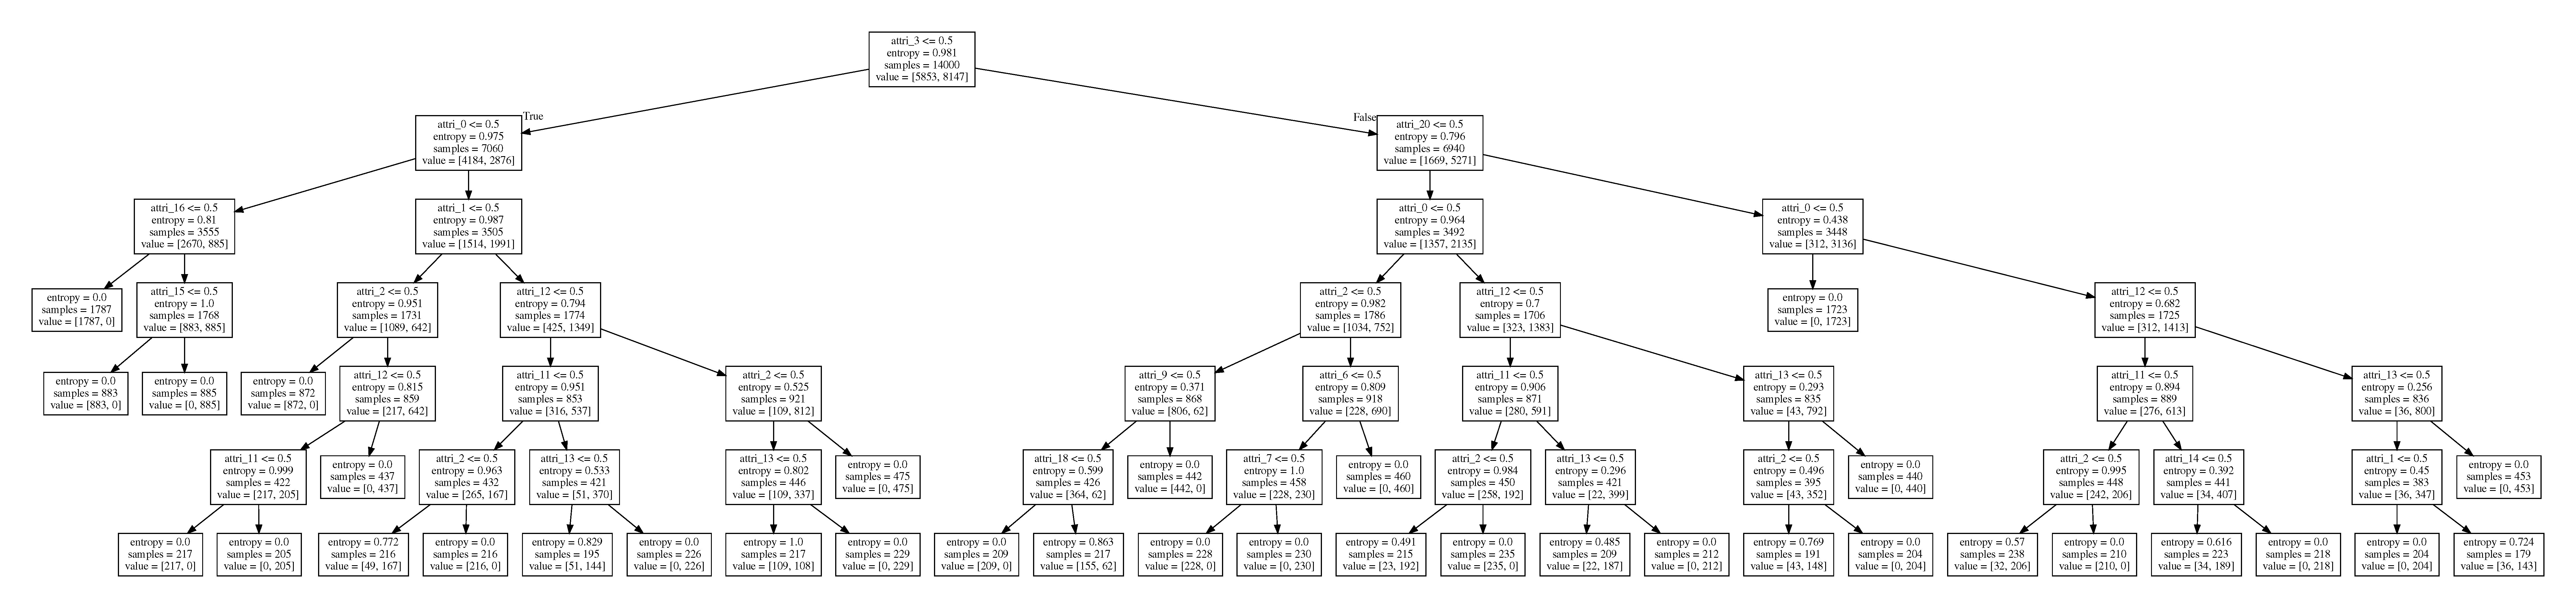
\includegraphics[width=550pt]{decision_tree_depth_m2_6.png}
        \caption{max-depth=6}
    \end{center}
\end{figure}


\begin{figure}[H]
    \begin{center}
        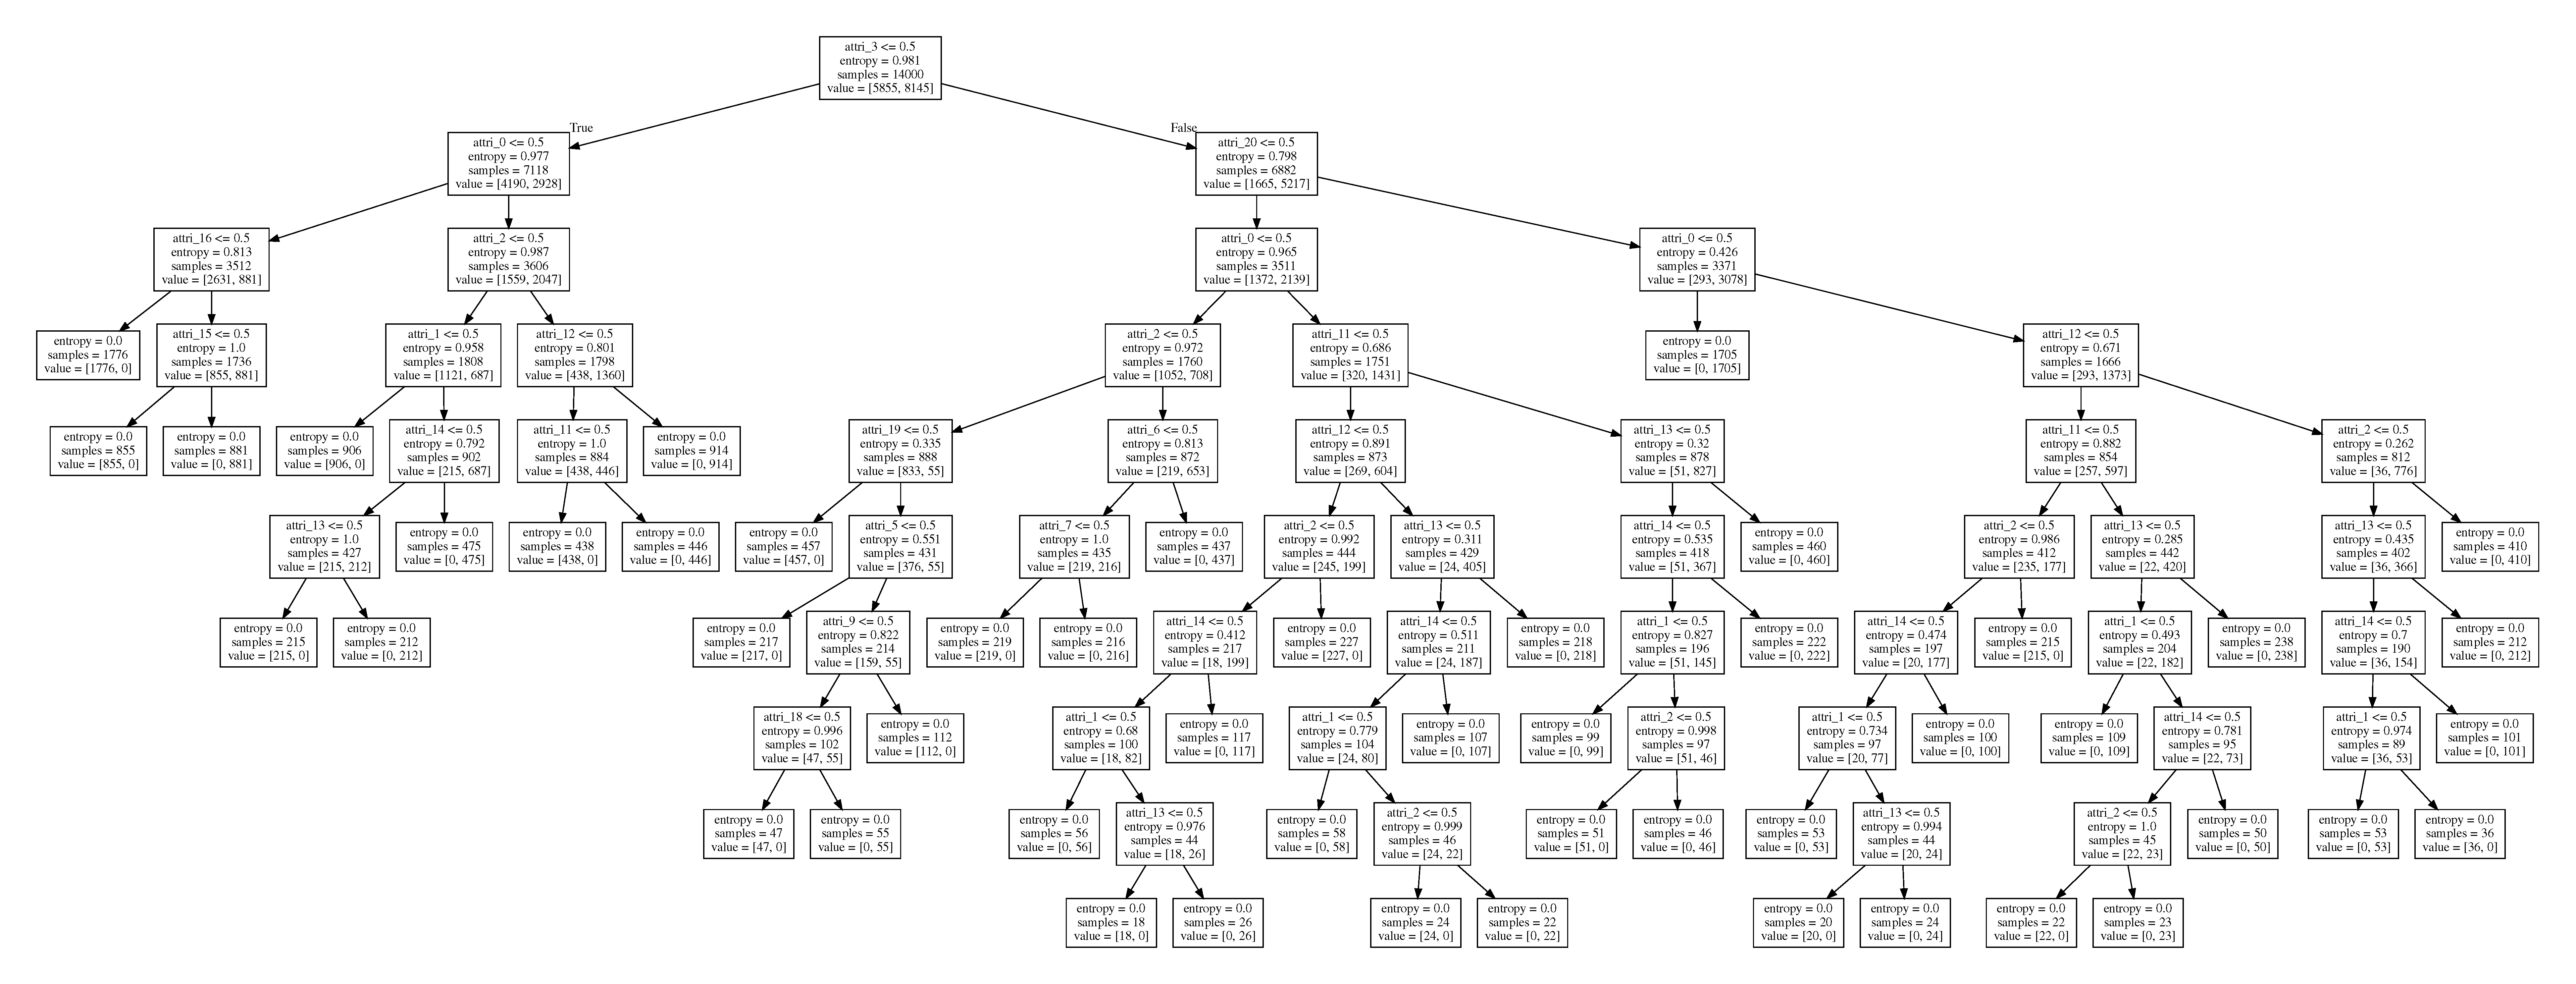
\includegraphics[width=550pt]{decision_tree_depth_m2_7.png}
        \caption{max-depth=7}
        \label{fig:123}
    \end{center}
\end{figure}

\section*{Discussion}
\label{sec:Discussion)}
\bookmark[level=chapter,page=\arabic{page}]{Discussion}

由視覺化的結果來看可以發現許多有趣的現象,照理來說即使深度不同,每個節點的feature應該要一致才對,後來才發現是我在程式的部分是讓每個深度的結構從新產生新的一組隨數據所造成的,而這樣的結果讓我發現即使是同一套規則下所產的數據,在不一樣的特徵數量分布下會使得決策樹會有不一樣的樹狀結構,因為若某個特徵在數量上的不同會導致不太一樣的gini值或entropy值。而在這我所設計的套規則下,就有幾個特徵所影響的權重蠻相近的,所以一當資料不同時就有可能造成節點順序上的不同。\\

由最後一張圖得知,即使在樹結構上相差甚遠,還是依然可以得到完全一樣的答案,但這在思考脈絡卻與原先的設計完全不一樣。由此可見,在這樣的特徵與對應的結果下,自己的設計規則可能並不是唯一的解,就像最後倒數兩張的情況一樣,一個非常接近我原本的設計,而另一個則是完全不一樣的結構,但兩個的準確率都是全對,但這樣的結果是非常有可能會導致overfitting的狀況,一但有雜訊的輸入,所產生的結果就會不盡理想,並不是每個情況都是成立的。\\



\bibliography{./reference} \label{sec:references}
\bookmark[level=chapter,page=\arabic{page}]{References}

\end{document}